\chapter{研究现状} \label{chap:related}
本文根据在视频目标跟踪中使用方法的不同将视频目标跟踪方法分为传统的基于相关滤波的视频目标跟踪方法和基于深度学习的视频目标跟踪方法。
其中,基于相关滤波的视频目标跟踪方法的...。近年来,深度学习方法在视频目标跟踪任务中的应用越来越广泛。基于深度学习的视频目标跟踪方法,尤其是基于卷积神经网络的视频目标跟踪方法,受到学术和工业界的广泛关注。接下来,本章将分别对传统的基于相关滤波的视频目标跟踪方法和基于深度学习的视频目标跟踪方法进行系统的介绍。
\section{基于传统相关滤波的跟踪器}
相关滤波跟踪的基本思想就是,设计一个滤波模板,利用该模板与目标候选区域做相关运算,最大输出响应的位置即为当前帧的目标位置。该跟踪器通过利用离散傅立叶变换以有效的方式利用了跟踪样本的所有空间偏移。
基于相关滤波的视频目标跟踪算法将空域内的密集搜索通过相关滤波的方式转化为频域内的点积运算,得益于快速傅里叶变换,在频域内高效进行表观建模,跟踪实时性好,能够达到很高的帧率。
Bolme 等 \cite{MOSSE} 首次将相关滤波于自适应目标跟踪相结合,提出 MOSSE 跟踪算法,该跟踪器以每秒 669 帧的速度运行,可以抵抗光照,比例,姿势和非刚性变形的变化。
CSK 跟踪器 \cite{Henriques2012ExploitingTC} 通过采用图像子窗口的循环结构并使用快速傅里叶变换(FFT)快速合并来自所有子窗口的信息,对 MOSSE 跟踪器进行了改进。此外, \cite{Henriques2012ExploitingTC} 表明,使用核技巧可以像在原始图像空间中一样高效地完成非线性空间中的分类。
\cite{Danelljan2014AdaptiveCA} 通过学习有关多维颜色属性的多通道滤镜来改进 CSK 跟踪器。为了避免由于颜色属性的高维而导致的计算开销,\cite{Danelljan2014AdaptiveCA} 提出了一种自适应维降技术,可以将原始的 11 维减少到只有 2 维。
后来,\cite{henriques2014high-speed} 为成千上万个已翻译补丁的数据集提出了一种分析模型。使用离散傅立叶变换将模型对角线化。此操作可以将存储和计算量减少几个数量级。

\section{基于深度学习的目标跟踪}
本章主要介绍基于深度学习的目标跟踪的研究现状,将基于深度学习的跟踪器划分为以下几种类别:基于深度学习的相关滤波跟踪器,基于生成对抗网络的跟踪器,基于图卷积网络的跟踪器,基于循环神经网络的跟踪器,基于孪生网络的跟踪器,基于强化学习的跟踪器,基于无监督学习的跟踪器,基于注意力机制的跟踪器和基于串并联或级联结构的跟踪器。

\subsection{基于深度特征的相关滤波跟踪器}
相关滤波跟踪器是传统跟踪器中的代表之一。传统的相关滤波跟踪器通常采用手工设计的特征或底层特征,这限制了相关滤波器的潜力。随着深度学习时代的到来,有很多相关滤波跟踪器尝试使用深度特征代替底层特征,并取得了性能的提升。[5]利用从深度卷积神经网络中提取的特征进行相关滤波的学习,来提高跟踪精度和鲁棒性。作者利用最后一个卷积层的输出对目标的语义信息进行编码,使得跟踪器对于目标的表观变化具有鲁棒性。但是,由于空间分辨率太粗糙,无法精确定位目标。相反,较浅的卷积层提供了更精确的定位。因此作者在每个卷积层上自适应学习相关滤波器,以对目标表观进行编码。在[6]中,作者在常规相关滤波跟踪器框架的基础上,提出了一种用于训练连续卷积滤波器的算法。作者采用隐式插值模型来解决连续空间域中的学习问题。该模型可实现对于多种分辨率的特征图的有效集成。此外,该方法能够进行亚像素定位,有利于提高跟踪的精确性。
\subsection{基于生成对抗网络的跟踪器}
生成对抗网络(GAN)可以通过CNN从随机噪声生成逼真的图像。 生成对抗网络包含两个子网,一个充当生成器,另一个充当判别器。 生成器旨在合成图像以欺骗判别器,而判别器则试图正确区分真实图像和生成器合成的图像。通过相互竞争来同时训练生成器和鉴别器。对抗学习的优势在于,所训练的生成器可以生成与训练样本相似的图像统计信息,从而使判别器无法区分。生成对抗网络的进步吸引了包括目标跟踪在内的各种计算机视觉应用的关注。在[7]中,作者利用生成对抗网络产生的样本辅助跟踪器的学习。文章指出,由于以下问题,现有视觉跟踪器的性能可能会受到限制:i)采用密集采样策略生成的正样本会降低样本的多样性;ii)即使收集到大规模的训练数据集,具有挑战性的训练数据也是有限的。作者提出了VITAL算法来通过对抗学习解决这两个问题。为了增加正样本,作者使用一个生成网络随机生成模板,这些模板用于自适应过滤输入特征以捕获各种表观变化。通过对抗学习获得的模板,可以提供最鲁棒的目标特征。此外,为了解决类别不平衡的问题,作者提出了一个高阶成本敏感损失,从而有助于训练分类网络。在[8]中,作者通过对抗生成学习产生难例正样本进行跟踪。具体来说,作者假设目标都位于流形上,因此,引入正样本生成网络(PSGN),通过遍历已构建的目标流形来采样大量训练数据。生成的各种目标图像可以丰富训练数据集并增强目标跟踪器的鲁棒性。为了使跟踪器对遮挡更加鲁棒,作者提出了一个变换网络,该网络可以生成用于跟踪算法的难例样本。
\subsection{基于图卷积网络的跟踪器}
图卷积神经网络(Graph Convolutional Network)是一种能对图数据进行深度学习的方法。在目标跟踪中,图卷积网络用于捕获目标样本的结构特征。在[9]中,作者指出时空信息可以用于增强目标表示,并且上下文信息对于目标的定位很重要。为了全面利用历史目标样本的时空结构并从上下文信息中受益,作者提出了一种用于高性能视觉跟踪的新型图卷积跟踪(GCT)方法。具体而言,GCT将两种类型的图卷积网络(GCN)合并到用于目标表观建模的孪生框架中。作者采用时空GCN来建模历史目标样本的结构化表示。而上下文GCN被设计为利用当前帧的上下文来学习用于目标定位的自适应特征。在[10]中,作者同样使用GCN模块来学习目标跟踪的结构特征。首先,作者利用双路径网络提取异构特征。然后,作者采用GCN模块来构建具有结构化信息的要素。
\subsection{基于循环神经网络的跟踪器}
循环神经网络(Recurrent Neural Network, RNN)是一类以序列(sequence)数据为输入,在序列的演进方向进行递归(recursion)且所有节点(循环单元)按链式连接的神经网络。RNN在建模序列数据方面引起了越来越多的关注。这些应用程序涵盖了多语言机器翻译[11],动作识别[12,13],场景标记[14,15],语音识别[16]等。最近,传统的RNN被归纳为更复杂的结构模型,例如二维RNN [17,18],多维RNN [19,20,21],树RNN [22,23]等。在目标跟踪中,可利用RNN建模目标的复杂远程依赖关系。RTT[24]尝试识别并利用那些对整个跟踪过程有益的可靠部分。为了解决遮挡并发现可靠的组件,RTT中使用了多方向递归神经网络,通过从多个方向遍历候选空间区域来捕获远程上下文线索。从RNN生成的置信度图用于抑制背景噪声,同时充分利用来自可靠部分的信息,来自适应地区分判别相关滤波器的学习。在[25]中,作者提出了一种能够将时间信息整合到模型中的实时目标跟踪器。该跟踪器不是专注于有限的一组目标或在测试时训练一个模型来跟踪特定的实例,而是在大量不同的目标上预先训练一个通用跟踪器,并进行实时的在线更新。
\subsection{基于孪生网络的跟踪器}
孪生网络是一种用于度量学习的有监督模型。孪生网络具有两个参数共享的子网络,可以学习两幅输入图像之间的特征相似性。由于优越的性能,基于孪生网络的跟踪器已经成为当前目标跟踪领域的主流。在SiamFC[26]中证明了使用孪生网络解决跟踪问题的有效性。具体来说,作者训练了一个孪生网络以在较大的搜索图像中定位模板图像。利用互相关操作以滑动窗口的方式获得目标位置的响应图,从而对目标进行实时定位。在SiamRPN[27]中,跟踪器由用于特征提取的孪生网络和包括分类分支和回归分支的region proposal子网络组成。受益于跟踪器的改进,传统的多尺度测试和在线微调可以被丢弃。SiamRPN++ \cite{SiamRPN++} 基于其在分类和状态估计分解中的成功经验,通过一种简单而有效的空间感知采样策略进一步突破了严格的翻译不变性的限制,并成功地训练了 ResNet 驱动的孪生跟踪器,从而显着提高了性能。除了这些基于锚的方法以外,还通过考虑无歧义评分,无目标目标规模/比率分布和估计质量评估准则,进一步设计了无锚跟踪器 SiamFC++ \cite{SiamFC++}。
\subsubsection{孪生网络跟踪器的模型自适应}
模型更新是传统目标跟踪算法中的重要一环。然而,流行的孪生跟踪器通常采用离线训练的模型而不进行模型更新。因此,有一些算法尝试在孪生网络中进行模型更新。
\subsection{基于强化学习的跟踪器}
强化学习(RL)的目标是学习一种通过最大化未来累积奖励来决定动作序列的策略。在[28]中,作者提出了一种新颖的跟踪器,该跟踪器顺序执行通过深度强化学习而学到的动作来进行控制。与使用深层网络的现有跟踪器相比,所提出的跟踪器旨在实现轻量级计算以及令人满意的跟踪精度。控制动作的深层网络使用各种训练序列进行了预训练,并在跟踪过程中进行了微调,以在线适应目标和背景变化。在[29]中,作者将跟踪形式化为部分可观察的决策过程(POMDP)来学习最佳决策策略。作者使用深度强化学习算法学习策略,这些算法仅在运动轨迹出现问题时才需要监督(奖励信号)。作者证明稀疏的奖励有利于快速地对海量数据集进行训练。
\subsection{基于无监督学习的跟踪器}
无监督学习(unsupervised learning)是机器学习的一种方法,没有给定事先标记过的训练样本,自动对输入的数据进行分类或聚类。常见的目标跟踪方法往往需要以监督方式进行训练,需要大量带注释的真实标签。手动注释往往是昂贵且费时的,而大量的未标记视频可在Internet上轻松获得。通过无监督学习,可以利用未标记的视频序列进行视觉跟踪。在[30]中,作者通过使用辅助自然图像,离线训练堆叠式去噪自动编码器,以学习对变化更鲁棒的通用图像特征。然后,将知识从离线培训转移到在线跟踪过程。在线跟踪网络由训练过的自动编码器(作为特征提取器)和一个附加的分类层构成。特征提取器和分类器都可以进行在线更新以适应运动目标的表观变化。在[31]中,作者提出了一种无监督的视觉跟踪方法。与使用大量有标签数据进行监督学习的现有方法不同,作者提出的CNN模型是在无监督的大规模无标签视频上进行训练的。作者的动机是,强大的跟踪器在前向和后向预测中均应有效(即,跟踪器可以在连续帧中向前定位目标并回溯到其在第一帧中的初始位置)。作者在一个孪生相关滤波网络上构建跟踪框架,该网络使用未标记的原始视频进行训练。同时,文中提出了一种多帧验证方法和一种成本敏感的损失函数,以促进无监督学习。
\subsection{对抗学习在视目标跟踪中的应用}
研究表明,卷积神经网络容易受到对抗攻击。在孪生神经网络中也是如此。
\subsection{基于注意力机制的跟踪器}
注意力机制首先用于神经科学领域[32]。它们已经扩展到其他领域,例如图像分类[33,34,35],姿态估计[36]等。在目标跟踪领域中,注意力机制有利于使网络的学习关注更有效的信息。	RASNet模型[37]在孪生跟踪框架内重新构造了相关过滤器,并引入了各种注意机制来适应模型而无需在线更新模型。通过利用离线训练的通用注意力,目标自适应的残差注意力以及通道特征注意力,RASNet不仅减轻了深度网络训练中的过拟合问题,而且具有更强的判别能力和适应性,从而提高了跟踪的性能。文中提出的深度架构是端到端训练的,充分利用了丰富的时空信息来实现强大的视觉跟踪。在[38]中,作者提出了一种具有注意力机制的新型跟踪框架,该机制通过选择相关过滤器的子集以提高鲁棒性和计算效率。滤波器的子集由深度注意力网络根据目标的动态属性进行自适应选择。该算法的贡献主要有:(1)引入注意力相关过滤器网络,该网络可以自适应跟踪动态目标。(2)利用注意力网络将注意力转移到最佳候选模块,并预测当前非活动模块的估计准确性。(3)扩大了相关滤波器的种类,涵盖目标漂移,模糊,遮挡,缩放变化和灵活的宽高比。(4)通过大量实验验证了视觉跟踪注意机制的鲁棒性和效率。
\subsection{基于串并联或级联结构的跟踪器}
SPM-Tracker[39]的基本思想是在两个单独的匹配阶段解决两个需求。在粗匹配(CM)阶段,通过通用训练增强了鲁棒性,而在精细匹配(FM)阶段,通过在线学习,增强了网络辨别力。 FM阶段的输入区域由CM阶段生成,因此这两个阶段串联连接。同时,这两个阶段也被并行连接,因为匹配分数信息和目标边框位置信息被融合以生成最终结果。这种创新的串并联结构充分利用了两个阶段的优势,并具有出色的性能。在[40]中,作者指出,最近流行的SiamRPN目标跟踪器在存在表观近似的干扰目标和目标剧烈变化的情况下会退化。为了解决这些问题,作者提出了一个多阶段跟踪框架,即孪生级联RPN(C-RPN),该框架由一系列来自孪生网络中不同层次的RPN组合而成。与以前的解决方案相比,C-RPN具有几个优点:(1)每个RPN在上一阶段都使用RPN的输出进行训练。这样的过程会关注难分的负采样,从而使训练样本更加均衡。因此,RPN在区分困难的背景(即类似的干扰因素)时将更具区分性。(2)提出了特征转移块(FTB)以充分利用多级特征,从而进一步使用高级语义和低级空间信息来改善C-RPN的辨别能力。(3)通过多步回归,C-RPN在多个阶段逐步调整每个RPN中目标的位置和形状,从而使定位更加准确。

\subsection{孪生网络跟踪器}
基于孪生跟踪器的网络结构首先在 SiamFC 被提出。SiamFC 的结构如图所示:

\begin{figure}
\centering
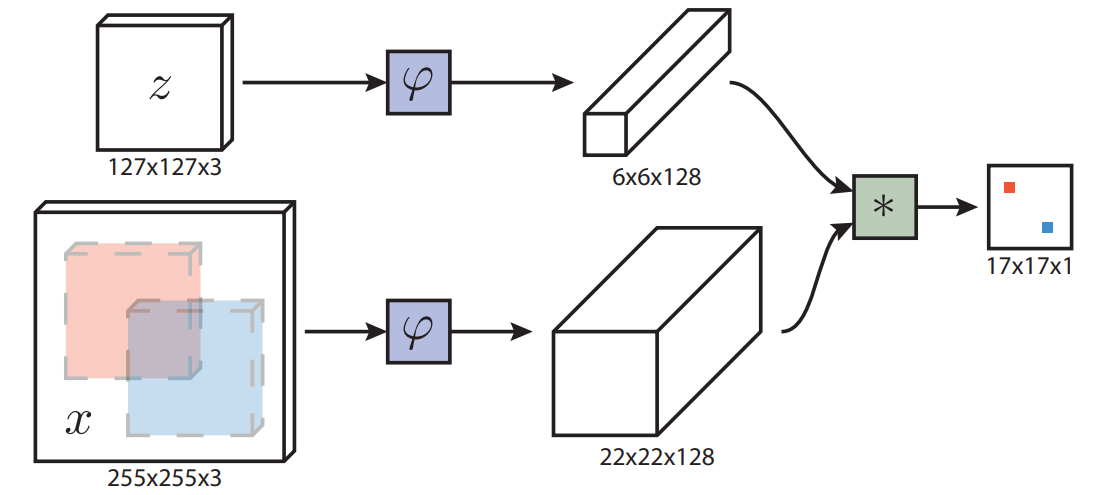
\includegraphics[width=0.75\textwidth]{Img/related/SiamFC.png}
\caption{SiamFC}
\end{figure}

\begin{figure}
\centering
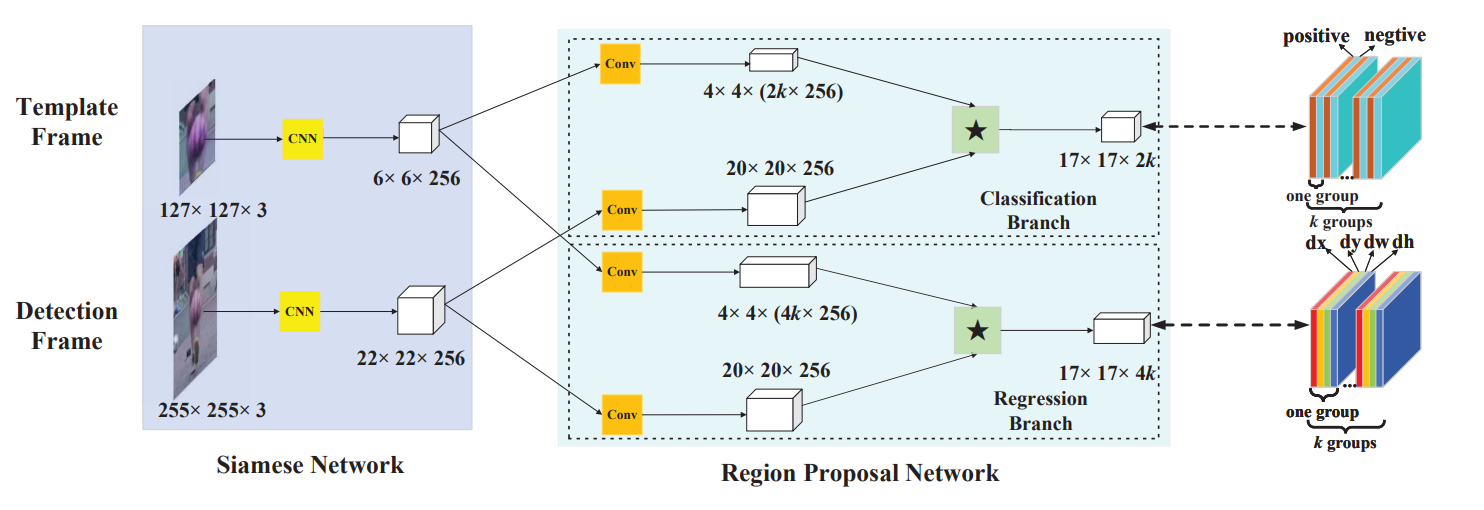
\includegraphics[width=0.75\textwidth]{Img/related/SiamRPN.png}
\caption{SiamRPN}
\end{figure}

\begin{figure}
\centering
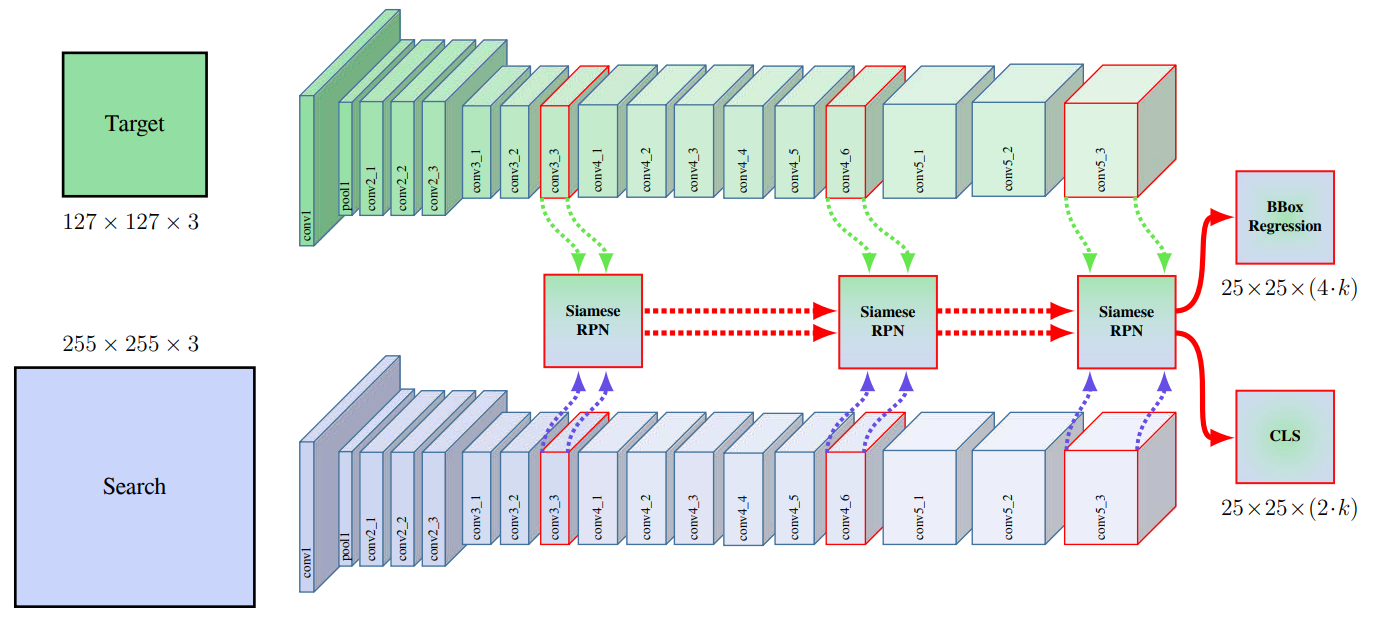
\includegraphics[width=0.75\textwidth]{Img/related/SiamRPN++.png}
\caption{SiamRPN++}
\end{figure}

\begin{figure}
\centering
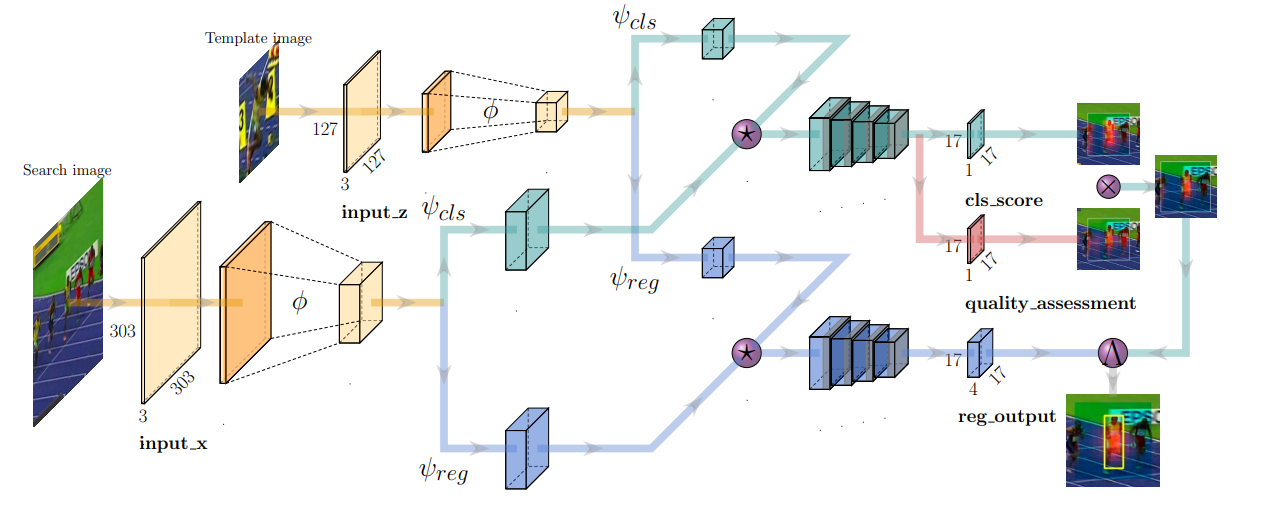
\includegraphics[width=0.75\textwidth]{Img/related/SiamFC++.png}
\caption{SiamFC++}
\end{figure}

\subsection{利用对抗信息对视频目标跟踪算法进行攻击}
